% Slides for Chapter 2 of the BARCS student guide: the calculations.
% Build in this folder: pdflatex barcs_slides_ch2.tex (run twice).
\documentclass[aspectratio=169,11pt]{beamer}
% Shared preamble for the BARCS student-guide slides (Beamer, metropolis).
% The slides follow the two-chapter textbook in ../chapter1 and ../chapter2:
% each section is one textbook step with the same title, and the worked
% examples use the same numbers. Short sentences, as in the textbook
% (ASD-STE100 style). No quiz: the quizzes stay in the textbook.
\usetheme[progressbar=frametitle,sectionpage=progressbar,numbering=fraction]{metropolis}
\usepackage[T1]{fontenc}
\usepackage{lmodern}
\usepackage{amsmath,amssymb}
\usepackage{booktabs}
\usepackage[most]{tcolorbox}
\usepackage{tikz}
\usetikzlibrary{arrows.meta,positioning}

\definecolor{barcsblue}{HTML}{0072B2}
\definecolor{barcsgreen}{HTML}{009E73}
\definecolor{barcsorange}{HTML}{D55E00}
\definecolor{barcsdark}{HTML}{1F3B4D}
\setbeamercolor{frametitle}{bg=barcsdark,fg=white}
\setbeamercolor{progress bar}{fg=barcsorange,bg=barcsdark!30}
\setbeamercolor{title separator}{fg=barcsorange}
\setbeamercolor{alerted text}{fg=barcsorange}
\setbeamercolor{normal text}{fg=black!85}

% The same three boxes as the textbook.
\newtcolorbox{symbols}[1][What the symbols mean]{colback=barcsblue!5,colframe=barcsblue,
  fonttitle=\bfseries\small,title=#1,boxrule=0.6pt,arc=2pt,left=4pt,right=4pt,top=2pt,bottom=2pt}
\newtcolorbox{worked}[1][]{colback=barcsgreen!6,colframe=barcsgreen!80!black,
  fonttitle=\bfseries\small,title=Worked example#1,boxrule=0.6pt,arc=2pt,left=4pt,right=4pt,top=2pt,bottom=2pt}
\newtcolorbox{remember}{colback=barcsorange!6,colframe=barcsorange,
  fonttitle=\bfseries\small,title=Remember,boxrule=0.6pt,arc=2pt,left=4pt,right=4pt,top=2pt,bottom=2pt}

\author{Prepared for Hyun-Hwan Jeong and Kyu-Won Lee}
\date{Companion slides to the student guide \quad$\cdot$\quad BARCS 0.2.1 \quad$\cdot$\quad Grades 7 to 9}

% The four-library example used in both chapters.
\newcommand{\datatable}{%
\begin{tabular}{lcrr}
\toprule
Library & Group & Guide count $K$ & Total count $N$\\
\midrule
1 & control & 180 & 1{,}000{,}000\\
2 & control & 240 & 1{,}200{,}000\\
3 & drug    & 120 & 1{,}000{,}000\\
4 & drug    &  80 &   800{,}000\\
\bottomrule
\end{tabular}}

\title{How BARCS Finds Important Genes}
\subtitle{Chapter 2: The calculations}

\begin{document}

\maketitle

\begin{frame}{The plan for Chapter 2}
\begin{columns}[T]
\begin{column}{0.55\textwidth}
\begin{enumerate}
\setcounter{enumi}{5}
\item[6.] How BARCS finds the best $\beta$ values
\item[7.] How BARCS measures the biological noise
\item[8.] Is the effect real?
\item[9.] Borrow information from other guides
\item[10.] Check the results with control guides
\item[11.] From guides to genes
\item[12.] Many genes and false discoveries
\end{enumerate}
\end{column}
\begin{column}{0.4\textwidth}
\begin{remember}
Each section has the same title as a step in Chapter~2 of the textbook. The
numbers are real BARCS 0.2.1 output for our example.
\end{remember}
\end{column}
\end{columns}
\end{frame}

%=====================================================================
\section{What you need from Chapter 1}
%=====================================================================

\begin{frame}{Our example and the key ideas}
\begin{columns}[T]
\begin{column}{0.47\textwidth}
\centering
\resizebox{\linewidth}{!}{\datatable}
\end{column}
\begin{column}{0.5\textwidth}
\footnotesize
\begin{itemize}
\item Proportions: 191 (control) and 111 (drug) per million. Fold change
  0.58.
\item Log-odds: $-8.56$ (control), $-9.10$ (drug).
\item Variance: $N \times \mu \times (1-\mu) \times \bigl(1 + (N-1) \times \rho\bigr)$;
  $\rho$ = correlation of two reads from one library.
\item Independent values: variances add. $\times c$: variance
  $\times\, c \times c$.
\item Design matrix $X$ rows: $(1,0)$, $(1,0)$, $(1,1)$, $(1,1)$.
\item Prediction $\eta$ = row of $X$ times $\beta$;
  $\mu = e^{\eta}/(1+e^{\eta})$.
\item $\beta_0$: control log-odds. $\beta_1$: effect of the drug.
\end{itemize}
\end{column}
\end{columns}
\end{frame}

%=====================================================================
\section{Step 6: How BARCS finds the best \texorpdfstring{$\beta$}{beta} values}
%=====================================================================

\begin{frame}{Guess, check, improve}
BARCS uses a loop: \alert{iteratively reweighted least squares} (IRLS).
\begin{enumerate}
\item \textbf{Guess.} Start with the simple log-odds of each group.
\item \textbf{Predict.} Use $X$ to predict $\eta$ and $\mu$ for each library.
\item \textbf{Measure the noise.} Find $\rho$ (Step 7).
\item \textbf{Weigh.} Less noise gives a larger \alert{weight}.
\item \textbf{Correct.} Calculate a \alert{working value} for each library.
\item \textbf{Improve.} Weighted averages give the new $\beta$ values.
\item \textbf{Repeat} until the $\beta$ values stop changing.
\end{enumerate}
\end{frame}

\begin{frame}{The working value: a straight-line step}
$\ln(0)$ does not exist, so BARCS uses a straight line for the log-odds.
\medskip

\small
\begin{tabular}{@{}l l l l@{}}
\toprule
Part & At $p = 0.2$ & At $p = 0.201$ & Change $\div$ 0.001\\
\midrule
$\ln(p)$ & $-1.60944$ & $-1.60445$ & $4.99 \approx 1 \div 0.2 = 5$\\
$-\ln(1-p)$ & $+0.22314$ & $+0.22439$ & $1.25 = 1 \div 0.8$\\
log-odds & $-1.38629$ & $-1.38006$ & $6.24 \approx 6.25$\\
\bottomrule
\end{tabular}
\normalsize
\[
\text{slope} = \frac{1}{p} + \frac{1}{1-p} = \frac{(1-p) + p}{p \times (1-p)}
 = \frac{1}{p \times (1-p)}
\]
\vspace{-0.4em}
\[
v_i = \eta_i + (K_i/N_i - \mu_i) \times \frac{1}{\mu_i \times (1-\mu_i)}
\]
{\small Start at the prediction $\eta_i$; step along the line by the distance
$K_i/N_i - \mu_i$.}
\end{frame}

\begin{frame}{Why weights? Weight $= 1 \div$ variance}
Two measurements of the same thing: variances 1 and 4.
\medskip

\begin{tabular}{@{}lll@{}}
\toprule
Weights & Variance of the average & \\
\midrule
equal (1 and 1) & $(1 + 4) \div (2 \times 2) = 1.25$ & \\
$1 \div 1 = 1$ and $1 \div 4 = 0.25$ & $1 \div (1 + 0.25) = 0.8$ & \alert{smaller}\\
\bottomrule
\end{tabular}
\medskip

\begin{remember}
Weight $= 1 \div$ variance gives the average with the smallest variance.
So BARCS uses $w_i = 1 \div (\text{variance of } v_i)$.
\end{remember}
\end{frame}

\begin{frame}{The weight from the variance of the working value}
\small
\renewcommand{\arraystretch}{1.3}\setlength{\tabcolsep}{4pt}
\begin{tabular}{@{}l l l@{}}
\toprule
Quantity & Formula & Library 1, iteration 1\\
\midrule
1. variance of $K_i$ & $N_i \times \mu_i \times (1-\mu_i) \times \bigl(1 + (N_i-1) \times \rho\bigr)$ & $190.87 \times 1.3841 = 264.19$\\
2. variance of $K_i/N_i$ & line 1 $\div (N_i \times N_i)$ & $2.642 \times 10^{-10}$\\
3. variance of $v_i$ & line 2 $\div \bigl(\mu_i \times (1-\mu_i)\bigr)^2$ & $0.007251$\\
4. weight $w_i$ & $1 \div$ line 3 & $137.90$\\
\bottomrule
\end{tabular}
\normalsize
\[
w_i = \frac{N_i \times N_i \times \bigl(\mu_i \times (1-\mu_i)\bigr)^2}
        {N_i \times \mu_i \times (1-\mu_i) \times \bigl(1 + (N_i-1) \times \rho\bigr)}
 = \frac{N_i \times \mu_i \times (1-\mu_i)}{1 + (N_i - 1) \times \rho}
\]
{\small Line 1: Chapter 1, Step 4. Line 2: divide by $N$ $\Rightarrow$
variance $\div\, N \times N$. Line 3: the step multiplies by the slope
$\Rightarrow$ variance $\times$ slope$^2$.}
\end{frame}

\begin{frame}{New $\beta$ values, and why a loop}
For our design matrix, weighted averages of the working values:
\[
\beta_0 = \frac{w_1 \times v_1 + w_2 \times v_2}{w_1 + w_2}, \qquad
\beta_0 + \beta_1 = \frac{w_3 \times v_3 + w_4 \times v_4}{w_3 + w_4}
\]
\begin{remember}
$w$ and $v$ use $\mu$; $\mu$ comes from $\beta$; $\beta$ comes from $w$ and
$v$. So BARCS guesses, then repeats until nothing changes.
\end{remember}
\end{frame}

\begin{frame}{Iteration 1: guess, predict, measure the noise}
\begin{worked}[ 10a: iteration 1]
\textbf{Guess.} Control log-odds $-8.563522$, drug log-odds $-9.104869$.

So $\beta_0 = -8.563522$ and $\beta_1 = -9.104869 - (-8.563522) = -0.541347$.

\medskip
\textbf{Predict.} Control $\mu = 0.000190909$. Drug $\mu = 0.000111111$.

\medskip
\textbf{Measure the noise.} Step 7 gives $\rho = 0.0000003841$.
\end{worked}
\end{frame}

\begin{frame}{Iteration 1: weigh and correct library 1}
\begin{worked}[ 10b: library 1]
\textbf{Weigh.}

Top: $1{,}000{,}000 \times 0.000190909 \times 0.999809 = 190.87$

Bottom: $1 + 999{,}999 \times 0.0000003841 = 1.3841$

Weight: $w_1 = 190.87 \div 1.3841 = 137.90$

\medskip
\textbf{Correct.}

$K_1/N_1 - \mu_1 = 0.000180 - 0.000190909 = -0.0000109$

$-0.0000109 \div 0.000190873 = -0.0572$

Working value: $v_1 = -8.5635 + (-0.0572) = -8.6207$
\end{worked}
\end{frame}

\begin{frame}{Iteration 1: improve}
\begin{columns}[T]
\begin{column}{0.48\textwidth}
\centering\small
\begin{tabular}{@{}lrrr@{}}
\toprule
Lib. & $w_i$ & $v_i$ & $w_i \times v_i$\\
\midrule
1 & 137.905 & $-8.62068$ & $-1188.84$\\
2 & 156.785 & $-8.51589$ & $-1335.16$\\
3 &  80.269 & $-9.02486$ &  $-724.42$\\
4 &  67.988 & $-9.20488$ &  $-625.82$\\
\bottomrule
\end{tabular}
\end{column}
\begin{column}{0.5\textwidth}
\begin{worked}[ 10c: new values]
\small
Control:\\ $(-1188.84 - 1335.16) \div 294.69 = -8.564929$

Drug:\\ $(-724.42 - 625.82) \div 148.257 = -9.107414$

$\beta_1 = -9.107414 - (-8.564929) = -0.542486$
\end{worked}
\end{column}
\end{columns}
\end{frame}

\begin{frame}{The next iterations}
\begin{center}
\begin{tabular}{crr}
\toprule
After iteration & $\beta_0$ & $\beta_1$\\
\midrule
0 (the guess) & $-8.563522$ & $-0.541347$\\
1 & $-8.564929$ & $-0.542486$\\
2 & $-8.564934$ & $-0.542492$\\
3 & $-8.564934$ & $-0.542492$\\
\bottomrule
\end{tabular}
\end{center}
After iteration 3 nothing changes. Final: $\beta_0 = -8.565$,
$\beta_1 = -0.542$.
\medskip
\begin{remember}
The weights move $\beta_1$ from $-0.5413$ to $-0.5425$. Library 2 has the
most reads and the least relative noise, so it counts the most.
\end{remember}
\end{frame}

%=====================================================================
\section{Step 7: How BARCS measures the biological noise}
%=====================================================================

\begin{frame}{Pearson residuals and the rule for \texorpdfstring{$\rho$}{rho}}
A \alert{Pearson residual} is the distance from the prediction in standard
deviations:
\[
r_i = \frac{K_i - N_i \times \mu_i}{\sqrt{N_i \times \mu_i \times (1-\mu_i) \times \bigl(1 + (N_i-1) \times \rho\bigr)}}
\]
\begin{remember}
BARCS chooses $\rho$ so that the squared Pearson residuals add up to the
degrees of freedom:
\[
r_1^2 + r_2^2 + r_3^2 + r_4^2 = \text{df}
\]
\end{remember}
\end{frame}

\begin{frame}{Why the sum should be the degrees of freedom}
\begin{itemize}
\item A Pearson residual is a distance in SDs. If the model is right, its
  square is 1 on average (variance $\div$ variance).
\item True $\mu$: four libraries $\Rightarrow$ the sum is about 4.
\item BARCS uses the fitted $\mu$. Each fitted $\beta$ pulls the
  prediction toward the data and takes away 1 on average:
  $4 - 2 = 2 = \text{df}$.
\end{itemize}
\begin{worked}[ computer check]
20{,}000 artificial guides like ours, with the true $\rho$:\\
true $\mu$: average sum 4.00;\quad fitted $\mu$: average sum 2.00.
\end{worked}
{\small So BARCS chooses $\rho$ to make the sum exactly df (a \emph{method of
moments}).}
\end{frame}

\begin{frame}{Start with \texorpdfstring{$\rho = 0$}{rho = 0}}
\begin{worked}[ 11]
\centering\small
\begin{tabular}{@{}lrrr@{}}
\toprule
Library & $(K - N \times \mu)^2$ & $N \times \mu \times (1-\mu)$ & Squared residual\\
\midrule
1 & $(-10.64)^2 = 113.21$ & 190.60 & 0.594\\
2 & $(+11.23)^2 = 126.16$ & 228.72 & 0.552\\
3 & $(+9.17)^2 = 84.14$   & 110.82 & 0.759\\
4 & $(-8.66)^2 = 75.03$   &  88.65 & 0.846\\
\midrule
  &  & Sum & 2.751\\
\bottomrule
\end{tabular}

\raggedright
The sum (2.751) is bigger than df $= 2$. So there is more noise than
counting noise: $\rho > 0$.
\end{worked}
\end{frame}

\begin{frame}{Guess and check for \texorpdfstring{$\rho$}{rho}}
\begin{columns}[T]
\begin{column}{0.42\textwidth}
\centering
\begin{tabular}{@{}rr@{}}
\toprule
$\rho$ & Sum\\
\midrule
0           & 2.751\\
0.0000001   & 2.506\\
0.0000002   & 2.302\\
0.0000003   & 2.129\\
\alert{0.000000386} & \alert{2.000}\\
0.0000005   & 1.851\\
\bottomrule
\end{tabular}
\end{column}
\begin{column}{0.54\textwidth}
\begin{itemize}
\item A larger $\rho$ makes the sum smaller.
\item BARCS stops when the sum equals 2: $\rho = 0.000000386$.
\item If the sum is 2 or less at $\rho = 0$, BARCS uses $\rho = 0$.
\end{itemize}
\begin{symbols}[Variance inflation]
\small $2.751 \div 2 = 1.376$: the guide has 1.38 times more noise than
counting noise alone (used in Step 9).
\end{symbols}
\end{column}
\end{columns}
\end{frame}

%=====================================================================
\section{Step 8: Is the effect real?}
%=====================================================================

\begin{frame}{The standard error}
The \alert{standard error} (SE) tells how much $\beta_1$ can change because
of noise. For our design matrix, it comes from the weights:
\[
W_{\text{control}} = w_1 + w_2, \quad W_{\text{drug}} = w_3 + w_4, \qquad
\text{SE}(\beta_1) = \sqrt{\frac{1}{W_{\text{control}}} + \frac{1}{W_{\text{drug}}}}
\]
\begin{worked}[ 13]
\small
Final weights: 137.524, 156.322, 79.955, 67.737.

$W_{\text{control}} = 293.846$, \quad $W_{\text{drug}} = 147.692$

$1/293.846 + 1/147.692 = 0.003403 + 0.006771 = 0.010174$

$\text{SE} = \sqrt{0.010174} = 0.101$
\end{worked}
\end{frame}

\begin{frame}{Where the SE formula comes from}
\footnotesize
\renewcommand{\arraystretch}{1.3}\setlength{\tabcolsep}{4pt}
\begin{tabular}{@{}r@{\;}l l@{}}
\toprule
& Step & Why\\
\midrule
1. & variance of $v_i = 1 \div w_i$ & definition of the weight\\
2. & $\beta_0 = \frac{w_1}{W_c} \times v_1 + \frac{w_2}{W_c} \times v_2$ & Step 6 ($W_c = w_1 + w_2$)\\
3. & var.\ of $\beta_0 = \bigl(\frac{w_1}{W_c}\bigr)^2 \times \frac{1}{w_1} + \bigl(\frac{w_2}{W_c}\bigr)^2 \times \frac{1}{w_2}$ & $\times c \Rightarrow$ variance $\times\, c \times c$; add\\
4. & $\phantom{\text{var.\ of }\beta_0} = \frac{w_1 + w_2}{W_c \times W_c} = \frac{1}{W_c}$ & one $w$ cancels in each part\\
5. & var.\ of $(\beta_0 + \beta_1) = 1 \div W_{\text{drug}}$ & same for the drug libraries\\
6. & var.\ of $\beta_1 = 1 \div W_c + 1 \div W_{\text{drug}}$ & difference; $(-1) \times (-1) = +1$, so variances add\\
7. & $\text{SE} = \sqrt{\text{line 6}} = \sqrt{0.003403 + 0.006771} = 0.101$ & SE = SD of the estimate\\
\bottomrule
\end{tabular}
\end{frame}

\begin{frame}{The t value and the degrees of freedom}
\[
t = \frac{\beta_1}{\text{SE}}, \qquad
\text{df} = (\text{rows of } X) - (\text{columns of } X)
\]
\begin{itemize}
\item A $t$ value far from 0: the effect is large compared with the noise.
\item Fewer degrees of freedom: BARCS needs a bigger $t$.
\end{itemize}
\begin{center}
\begin{tabular}{lcccc}
\toprule
Degrees of freedom & 1 & 2 & 14 & very many\\
$|t|$ needed for $p < 0.05$ & 12.71 & 4.30 & 2.14 & 1.96\\
\bottomrule
\end{tabular}
\end{center}
\end{frame}

\begin{frame}{The p-value}
\begin{itemize}
\item The \alert{p-value}: if the true effect is 0, how often does noise
  alone give a $t$ this far from 0?
\item Small p-value: noise alone seldom gives such a result. The usual limit
  is 0.05.
\end{itemize}
\begin{worked}[ 14: testing the effect]
\small
\begin{enumerate}
\item $t = -0.542 \div 0.101 = -5.38$
\item $X$ has 4 rows and 2 columns: $\text{df} = 2$
\item df $= 2$ needs $|t| > 4.30$. Our $|t| = 5.38$. So $p < 0.05$.
\item Exact p-value: $p = 0.033$
\end{enumerate}
\end{worked}
\end{frame}

\begin{frame}{Degrees of freedom come from libraries}
\begin{remember}
The degrees of freedom come from the number of libraries, not from the
number of reads.

A library with 100 million reads still counts as one row of $X$.
\end{remember}
\end{frame}

%=====================================================================
\section{Step 9: Borrow information from other guides}
%=====================================================================

\begin{frame}{Moderation: a weighted vote}
\begin{itemize}
\item 2 degrees of freedom give an unreliable noise estimate.
\item A screen has thousands of guides with similar noise.
\item BARCS averages the guide's own inflation with the typical inflation.
\end{itemize}
\[
\text{moderated} = \frac{\text{df} \times \text{own} + d_0 \times \text{typical}}{\text{df} + d_0}
\]
\begin{symbols}
\small $d_0$: the \alert{prior degrees of freedom}, the votes of the typical
value. BARCS calculates it from all the guides.
\end{symbols}
\end{frame}

\begin{frame}{Worked example: moderation with simple numbers}
\begin{worked}[ 15]
A guide has df $= 3$ and own inflation 4.0. Typical inflation 1.5 with
$d_0 = 12$.
\[
\frac{3 \times 4.0 + 12 \times 1.5}{3 + 12} = \frac{12 + 18}{15}
 = \frac{30}{15} = 2.0
\]
The value moves from 4.0 toward 1.5 and stops at 2.0.
\end{worked}
\end{frame}

\begin{frame}{What moderation does to our guide}
\begin{columns}[T]
\begin{column}{0.42\textwidth}
\small
BARCS uses the moderated value to:
\begin{enumerate}
\item multiply the SE by $\sqrt{\text{moderated} \div \text{own}}$
  (variance $\propto$ inflation; SE $=$ $\sqrt{\text{variance}}$; own
  below 1 counts as 1)
\item recalculate $t$
\item use $\text{df} + d_0$ degrees of freedom
\end{enumerate}
BARCS moderates when it has 50 or more usable guides.
\end{column}
\begin{column}{0.55\textwidth}
\begin{worked}[ 16]
\small
Own inflation 1.376, df $= 2$. Typical 1.5, $d_0 = 12$.

Moderated: $(2 \times 1.376 + 12 \times 1.5) \div 14 = 1.482$

SE factor: $\sqrt{1.482 \div 1.376} = 1.038$

New SE: $0.101 \times 1.038 = 0.105$

New $t$: $-0.542 \div 0.105 = -5.18$, \ df $= 14$

New p-value: 0.00014
\end{worked}
\end{column}
\end{columns}
\end{frame}

%=====================================================================
\section{Step 10: Check the results with control guides}
%=====================================================================

\begin{frame}{Non-targeting control guides}
\begin{itemize}
\item \alert{Control guides} switch off no gene. Their true effect is 0.
\item About 5\% of them should get $p < 0.05$ by chance.
\item More than that: the noise model is too small. BARCS makes the tests
  wider.
\end{itemize}
\begin{worked}[ 17: the scale factor]
\small
100 control guides: we expect 5 with $p < 0.05$, but 15 have it.

95 of the 100 control guides have $|t|$ below 2.47. The table says 1.96.

Scale factor: $2.47 \div 1.96 = 1.26$. BARCS divides every $t$ by 1.26:
$t = 3.5$ becomes $3.5 \div 1.26 = 2.78$.
\end{worked}
\small The scale factor is never less than 1. Calibration only makes results
more careful.
\end{frame}

%=====================================================================
\section{Step 11: From guides to genes}
%=====================================================================

\begin{frame}{The Stouffer method}
\begin{enumerate}
\item Change each guide's p-value into a \alert{z score}. The sign follows
  the effect.
\item Add the z scores.
\item Divide by the square root of the number of guides, $m$.
\end{enumerate}
\[
Z_{\text{gene}} = \frac{z_1 + z_2 + \cdots + z_m}{\sqrt{m}}
\]
{\small Why $\sqrt{m}$: each $z$ has variance 1, so the sum has variance $m$;
dividing by $\sqrt{m}$ divides the variance by $m$ $\Rightarrow$ variance 1
again.}
\begin{center}
\small
\begin{tabular}{lccccc}
\toprule
Two-sided p-value & 0.317 & 0.134 & 0.046 & 0.012 & 0.0027\\
$z$ score & 1.0 & 1.5 & 2.0 & 2.5 & 3.0\\
\bottomrule
\end{tabular}
\end{center}
\end{frame}

\begin{frame}{Worked examples: combining guides}
\begin{columns}[T]
\begin{column}{0.48\textwidth}
\begin{worked}[ 18: three guides]
\small
p-values 0.046, 0.134, 0.012 give $z$ = 2.0, 1.5, 2.5.
\[
Z = \frac{2.0 + 1.5 + 2.5}{\sqrt{3}} = \frac{6.0}{1.732} = 3.46
\]
$p = 0.00053$. Together, the guides give strong evidence.
\end{worked}
\end{column}
\begin{column}{0.48\textwidth}
\begin{worked}[ 19: shared noise]
\small
Guides can share noise (\alert{guide correlation} $r$). Squares and pairs
(Chapter 1): $m$ squares $+$ $m \times (m-1)$ pairs $\times\, r$. Bottom:
$\sqrt{m + m \times (m-1) \times r}$.

With $r = 0.1$: $\sqrt{3 + 6 \times 0.1} = \sqrt{3.6} = 1.897$.

$Z = 6.0 \div 1.897 = 3.16$, \ $p = 0.0016$.
\end{worked}
\end{column}
\end{columns}
\end{frame}

%=====================================================================
\section{Step 12: Many genes and false discoveries}
%=====================================================================

\begin{frame}{Why we need a false discovery rate}
\small
\begin{itemize}
\item 20{,}000 genes with $p < 0.05$: about 1{,}000 pass by chance.
\item \alert{False discovery rate} (FDR): the expected fraction of false
  results in the list of hits.
\end{itemize}
\textbf{Idea:} with no effect, p-values are spread evenly from 0 to 1. Of
20{,}000 such genes, about $20{,}000 \times 0.001 = 20$ get $p \le 0.001$.
If 100 genes have $p \le 0.001$, about $20 \div 100 = 0.2$ of them are false.

\textbf{Benjamini--Hochberg method:}
\begin{enumerate}
\item Sort the genes by p-value and give them ranks.
\item Calculate $p \times (\text{number of genes}) \div \text{rank}$.
\item From the bottom up, replace a value with the value below it if that
  value is smaller.
\end{enumerate}
\end{frame}

\begin{frame}{Worked example: FDR for five genes}
\begin{worked}[ 20]
\centering\small
\begin{tabular}{@{}cccll@{}}
\toprule
Gene & Rank & $p$ & $p \times 5 \div \text{rank}$ & FDR\\
\midrule
A & 1 & 0.001 & $0.001 \times 5 \div 1 = 0.005$ & 0.005\\
B & 2 & 0.008 & $0.008 \times 5 \div 2 = 0.020$ & 0.020\\
C & 3 & 0.039 & $0.039 \times 5 \div 3 = 0.065$ & 0.051 (from D)\\
D & 4 & 0.041 & $0.041 \times 5 \div 4 = 0.051$ & 0.051\\
E & 5 & 0.600 & $0.600 \times 5 \div 5 = 0.600$ & 0.600\\
\bottomrule
\end{tabular}

\raggedright
FDR $< 0.05$: genes A and B. \quad FDR $< 0.10$: genes A, B, C and D.
\end{worked}
\end{frame}

%=====================================================================
\section{Two special cases}
%=====================================================================

\begin{frame}{Zero reads and very large changes}
\begin{columns}[T]
\begin{column}{0.48\textwidth}
\begin{block}{A guide with zero reads}
\small
0 reads in all control libraries means log-odds $= \ln(0)$, which does not
exist. Older BARCS removed the guide. BARCS 0.2.1 first adds less than one
read (the \alert{Firth correction}) and keeps it.
\end{block}
\end{column}
\begin{column}{0.48\textwidth}
\begin{block}{A very large change}
\small
A guide that grows hundreds of times can make the usual test fail: the SE
grows faster than the effect. The \alert{likelihood-ratio test} compares
the fit with and without the effect. \texttt{test = "auto"} uses it only
for such guides.
\end{block}
\end{column}
\end{columns}
\end{frame}

%=====================================================================
\section{Summary: the full path}
%=====================================================================

\begin{frame}{From counts to a list of genes}
\begin{center}
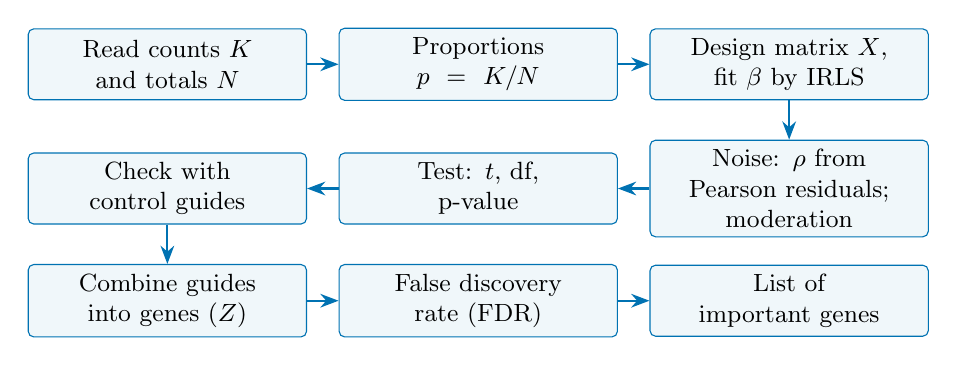
\begin{tikzpicture}[node distance=5mm and 4mm,
  box/.style={draw=barcsblue,fill=barcsblue!6,rounded corners=2pt,
              align=center,minimum height=9mm,text width=3.3cm,font=\small},
  arr/.style={-{Stealth},thick,barcsblue}]
\node[box] (a) {Read counts $K$\\and totals $N$};
\node[box,right=of a] (b) {Proportions\\$p = K/N$};
\node[box,right=of b] (c) {Design matrix $X$,\\fit $\beta$ by IRLS};
\node[box,below=of c] (d) {Noise: $\rho$ from\\Pearson residuals;\\moderation};
\node[box,left=of d] (e) {Test: $t$, df,\\p-value};
\node[box,left=of e] (f) {Check with\\control guides};
\node[box,below=of f] (g) {Combine guides\\into genes ($Z$)};
\node[box,right=of g] (h) {False discovery\\rate (FDR)};
\node[box,right=of h] (i) {List of\\important genes};
\draw[arr] (a)--(b); \draw[arr] (b)--(c); \draw[arr] (c)--(d);
\draw[arr] (d)--(e); \draw[arr] (e)--(f); \draw[arr] (f)--(g);
\draw[arr] (g)--(h); \draw[arr] (h)--(i);
\end{tikzpicture}
\end{center}
\end{frame}

\begin{frame}{The symbols of Chapter 2}
\centering\footnotesize\renewcommand{\arraystretch}{0.95}
\begin{tabular}{@{}lll@{}}
\toprule
Symbol & Meaning & Value in our example\\
\midrule
$w$ & weight of a library in the fit & 137.5 (library 1)\\
working value & prediction plus correction & $-8.621$ (library 1)\\
Pearson residual & distance from the prediction in SDs & $-0.65$ (library 1)\\
inflation & noise compared with counting noise & 1.376\\
SE & standard error of the effect & 0.101\\
$t$ & effect divided by SE & $-5.38$\\
df & rows of $X$ minus columns of $X$ & $4 - 2 = 2$\\
p-value & chance of this result if the effect is 0 & 0.033\\
$d_0$ & prior degrees of freedom (votes) & 12\\
$z$, $Z$ & z score of a guide, of a gene & 3.46\\
$m$ & number of guides for a gene & 3\\
$r$ & guide correlation (shared noise) & 0.1\\
FDR & expected fraction of false hits & 0.005 for gene A\\
\bottomrule
\end{tabular}
\end{frame}

\end{document}
